\chapter{Introduction}
\label{chp:introduction}
%--------------
\section{Research questions}
This desktop study addresses conceptual issues at the intersection of tide prediction and mesoscale oceanography, with practical implications for operational sea level forecasting practice. 
In contrast to the canonical numerical approach to coastal sea level that broadly pursues  ever-higher resolution simulations, this work turns to focus on the less-studied but relevant value offered by established operational systems; especially at the ocean mesoscale. Addressing the representation of sea level at the intersection of existing systems is important for building the foundations of future multi-model seamless forecasting services.


Motivation for the study originates from within the Australian Bureau of Meteorology in the context of the ongoing global trend towards so-called ``seamless'' services from operational agencies.   The data and systems described reflect this Australian setting.

In plain language, the following series of questions describe the research problems specifically addressed in chapters \ref{chp:aggregate}, \ref{chp:waveguide} and \ref{chp:tideFlavours}.

\emph{%
Is the operationalisation of high resolution coastal simulations a prerequisite for providing regular sea level forecasts?  Despite comparatively low coastal resolution, can a mesoscale ocean forecast directly provide useful prognosis of non-tidal coastal sea level and with what limitations? }



\emph{Are point-by-point tide-gauge observations the only relevant basis on which to compare and assess heterogeneous sea level forecast simulations? 
Why is the role of coastally trapped waves prominent in the oceanographic literature but seemingly absent from operational forecasting?}



\emph{Has numerical simulation rendered conventional tide prediction redundant for operations?  How can the unique traditional function of tide prediction compliment nominally non-tidal ocean forecasts and future seamless prediction systems? 
}


%--------------------------------------------------
\subsection{Data sources and terminology}
This study is intentionally based on data from within the Australian Bureau of Meteorology.
Operational archives of forecast system output, real-time observations and tidal analysis parameters are the primary data sources. In general these sources are not openly and directly published and are thus unfortunately not all easily accessible for independent research. However, the data does reflect the real basis of products issued by the Bureau under actual operating conditions.

Many of the sea level observations were supplied to the Bureau in near-real-time by external agencies under a variety of agreements that generally cover forecasting and research purposes.   Of special note these agencies include: New South Wales Manly Hydraulics Laboratory, the Queensland Government Department of Environment, Land and Water and Ports Australia.
These operational observations differ from typical research quality archives with respect to the type and level of quality control measures that are applied.   As a consequence this operational data is not guaranteed to be reported relative to a constant reference and can be susceptible to contamination with influences such as communication drop-outs and glitches.  Handling of observational quality issues like these is however fundamental to the operational setting as is discussed in the body of this manuscript. 


Table \ref{table:jargon} presents a brief summary of some key terminology and acronyms used in throughout this document.   Mostly these terms are are introduced and described in the body of the text but are highlighted here for reference and clarity.
\begin{table}[h]\centering
    \begin{tabular}{ |p{3cm}|p{11cm}| }
    \hline
    Term & Description  \\
    %-----------
    \hline
    Sea level & Generally ``still water level''; observed or simulated elevation of the ocean water surface; time scale range hours to weeks.\\
    %-----------
    \hline
    Tide & Sea level component somehow associated with the \ATGP{}; exposition of details and differing implications are taken up in section \ref{sec:tidesOverview}\\
    %-----------
    \hline
    \ATGP{} & Astronomical Tide Generating Potential, abstract definition of the time varying components of gravitational forces driving ocean tides as a Newtonian potential field.\\
    %-----------
    \hline
    Operational & Part of the regular or routine sustained daily production cycle of a service organisation;  in contrast to idealised,academic or historical re-analysis data and simulations.\\
    %-----------
    \hline
    Bluelink OceanMAPS & Mesoscale ocean forecasting system at the Australian Bureau of Meteorology; one component of the wider Bluelink ocean forecasting collaboration of the Australian CSIRO, Navy and Bureau of Meteorology.\\
    %-----------
    \hline
    Insitu & In place or undertaken directly at some place; with regard observations from fixed position instruments in particular. \\
    %-----------
    \hline
    Seamless &  Consistent and without discontinuities across multiple timescales; especially with regard to numerical forecasts and services built from a variety of sources. \\
    %-----------
    \hline
    \end{tabular}
    \caption{Select nomencalture}
    \label{table:jargon}
\end{table}


%--------------------------------------------------
\section{Observable sea level and forecasts}

Sea level plays a unique role in physical oceanography and forecasting thanks at least in part to the fact that it is actually observable \citep{Wilson:2010hy}. 
Variations in coastal \emph{still water level} \citep{Pugh:2014di} reflect a diverse range of hydrodynamic phenomena operating across time and length scales.   Furthermore the relative significance of the pheneomena vary greatly in space and time.
\citet{10.1007/s10712-019-09531-1} recently reviewed this diverse mix of physical phenomena present in the observations and note that ``\textit{it is mistake to think that coastal sea level variability always has a ‘local’ forcing (although it often does).}''. 
Figure \ref{fig:sealevelScales} provides a schematic summary of the physical time and length scales of broad classes of these phenomena that contribute to ocean water level variations, taking inspiration from similar diagrams in \citet{10.1007/s10712-019-09531-1} and \citet{Chelton:2001ws}.
%-----------------------------
\begin{figure}[H]\centering
  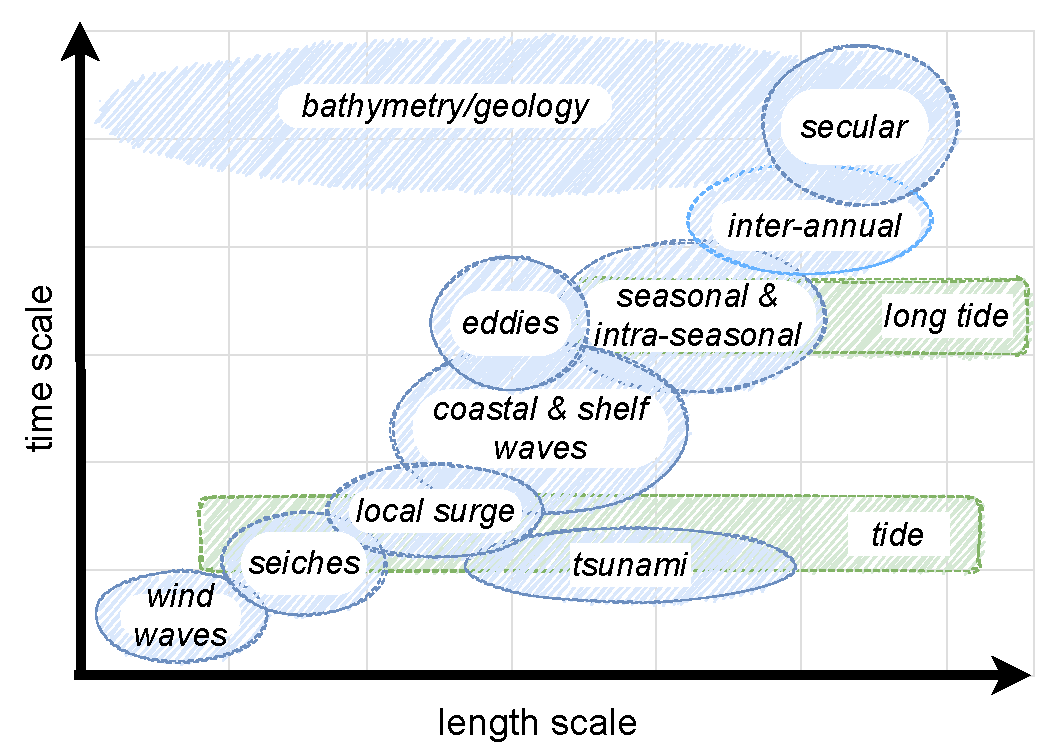
\includegraphics[width=\figwidthFull]{figures/diagrams/scales_time_length.pdf}
  \caption{Schematic indication of the relative time and length scales of a range of physical processes contributing to observable coastal sea level.}
  \label{fig:sealevelScales}
\end{figure}
%-----------------------------
The visual differentiation of tides from the other phenomena in Figure \ref{fig:sealevelScales} is intentional.  Tides have unique properties; but exactly what is designated as tidal in an operational context can be more ambiguous than first impressions imply. This topic is unpacked further in section \ref{sec:tide_intro}. Tides in the schematic are seen to span from very short to very long length-scales but at more restricted frequencies than other phenomena.    Furthermore, the long period tides are are shown separately in anticipation of a later discussion of how these species are potentially problematic in some forecasting applications.

How the varying balance of phenomena is expressed in observed sea level is illustrated by the spectra shown in Figure \ref{fig:obsSpectraEg} for two Australian locations.   Variability at nominally tidal frequencies is a striking feature at nearly all coastal locations;  ``the [tidal] constituent lines emerge from the noise background as trees from the grass'' \citep{godin:1972}.
Observed power at tidal frequencies does not however provide a direct attribution to tidal forcing and the extent to which this matters for forecasting applications is a conceptual theme addressed in chapter \ref{chp:tideFlavours}.
%-----------------------------
\begin{figure}[H]\centering
    \begin{subfigure}[b]{\figwidthFull}
        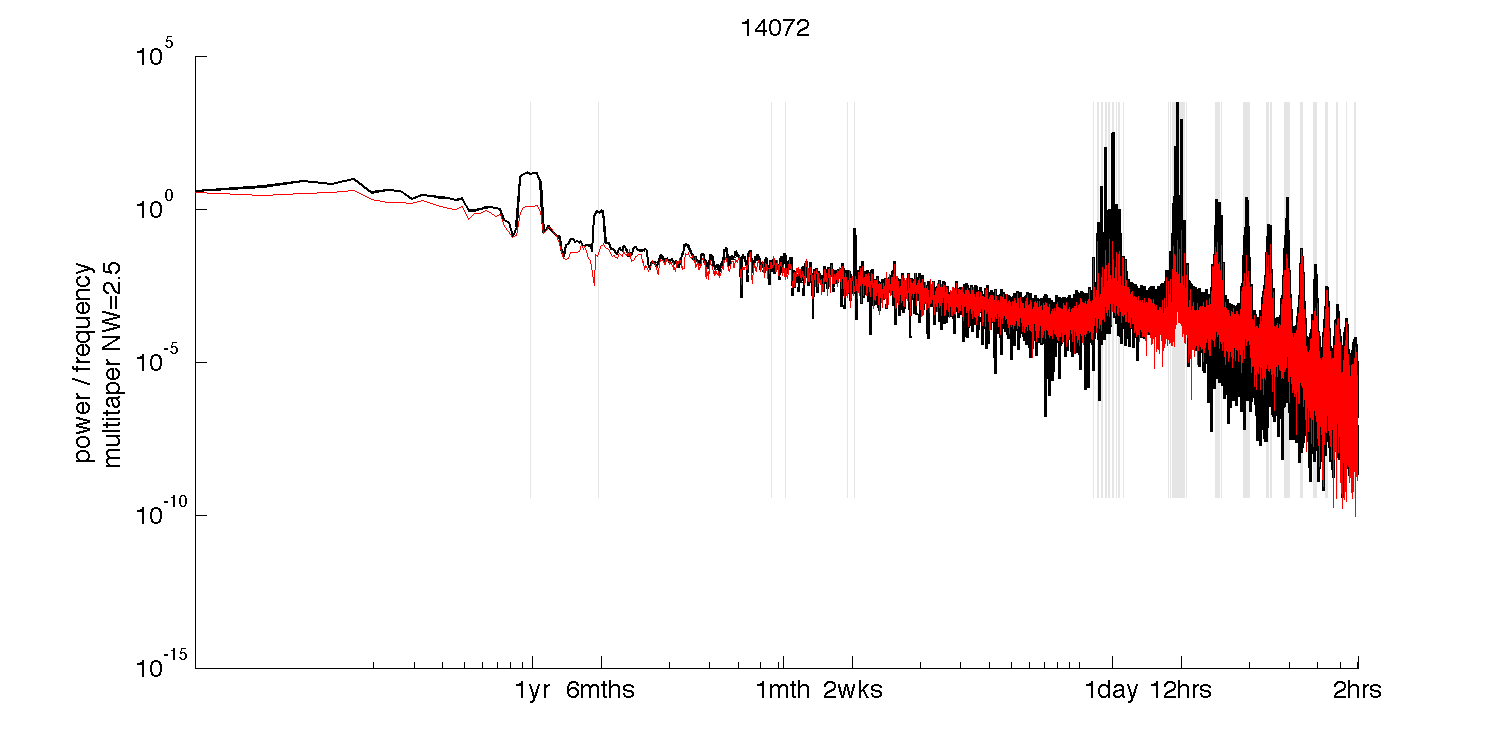
\includegraphics[trim={0 0 0 1cm},clip,width=\textwidth]{figures/plots/plot_14072.png} 
        \caption{Darwin in Northern Australia - large diurnal tide}
    \end{subfigure}
    
    \begin{subfigure}[b]{\figwidthFull}
        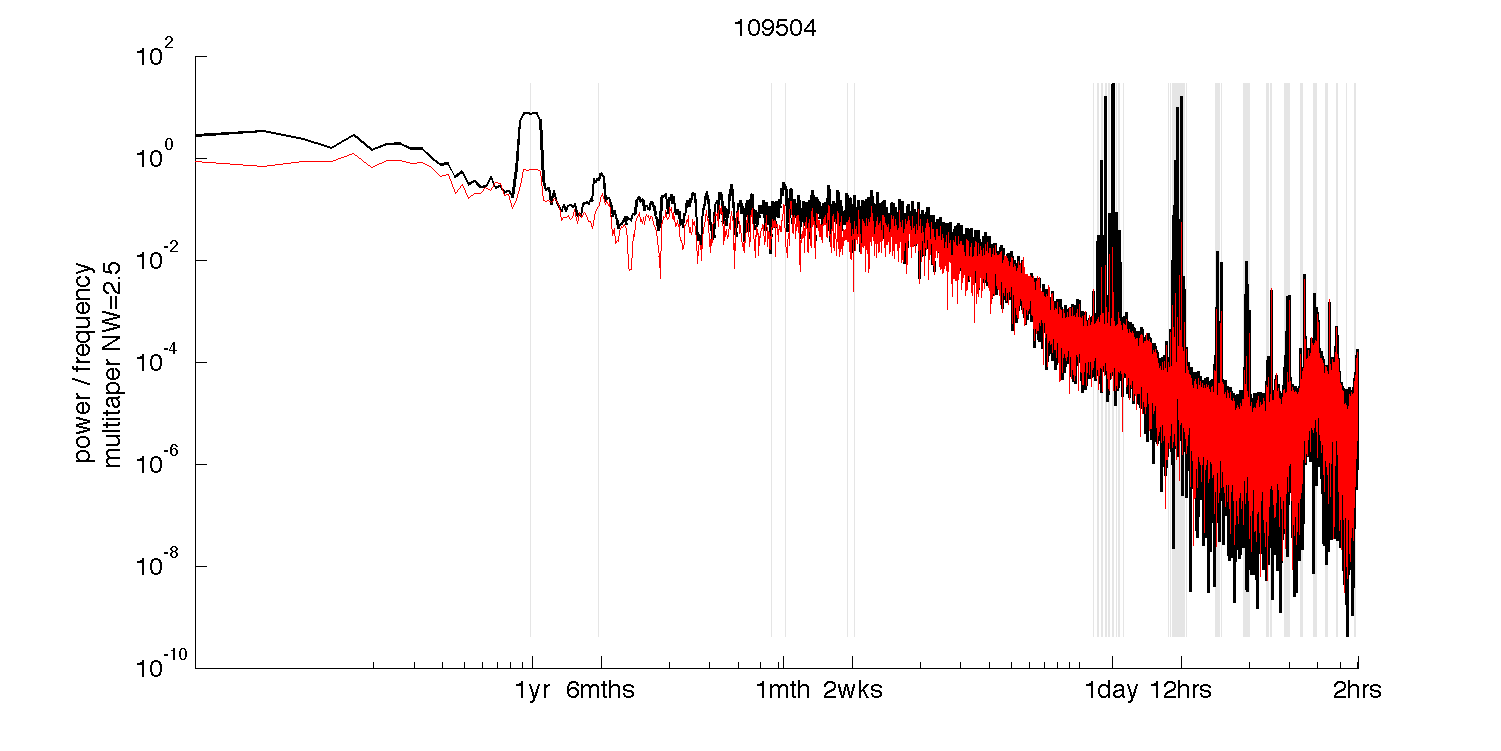
\includegraphics[trim={0 0 0 1cm},clip,width=\textwidth]{figures/plots/plot_109504.png} 
        \caption{Esperence in Southern Australia - powerful synoptic signal}
    \end{subfigure}
    \caption{Spectral estimates from two coastal tide gauges. Hourly data, black = observations, red = tidal residual, nominally tidal frequencies are shown with shading. An example of a `mixed spectra' \citep{Percival:1998tw}, in the sense of that prominent tidal spectral lines appear to be embedded in a background continuum of coloured variability.}
    \label{fig:obsSpectraEg}
\end{figure}   
%-----------------------------

Quantified observations of sea level currently available for operational use fall into essentially two categories: (1) insitu and (2) remote.    Figure \ref{fig:sealevelObsCartoon} illustrates this difference schematically.

Insitu observations from coastal tide gauges are by far the most established and studied source.    The availability of tide gauge observations is intrinsically connected to the history of sea level study and the development of forecasting techniques; the longer view of which is covered in the history of \citeauthor{Cartwright:2000tt}.
Typical tide gauge instruments in fact measure the `air gap' between a sensor and the water surface from which a relative level is derived \citep{PCTMSL-sp9}. 
But the very nature of why and how tide gauges are installed raises a list of special characteristics relevant to operational forecasting. These characteristics are variously considered to add complication or insight for different applications. \citeauthor{10.1175/jtech-d-18-0203.1} put it simply that ``\textit{most tide gauges are limited to deep water or sheltered harbors and omit part of the natural total sea level variability at open coasts}''.   
%-----------------------------
\begin{figure}[H]\centering
  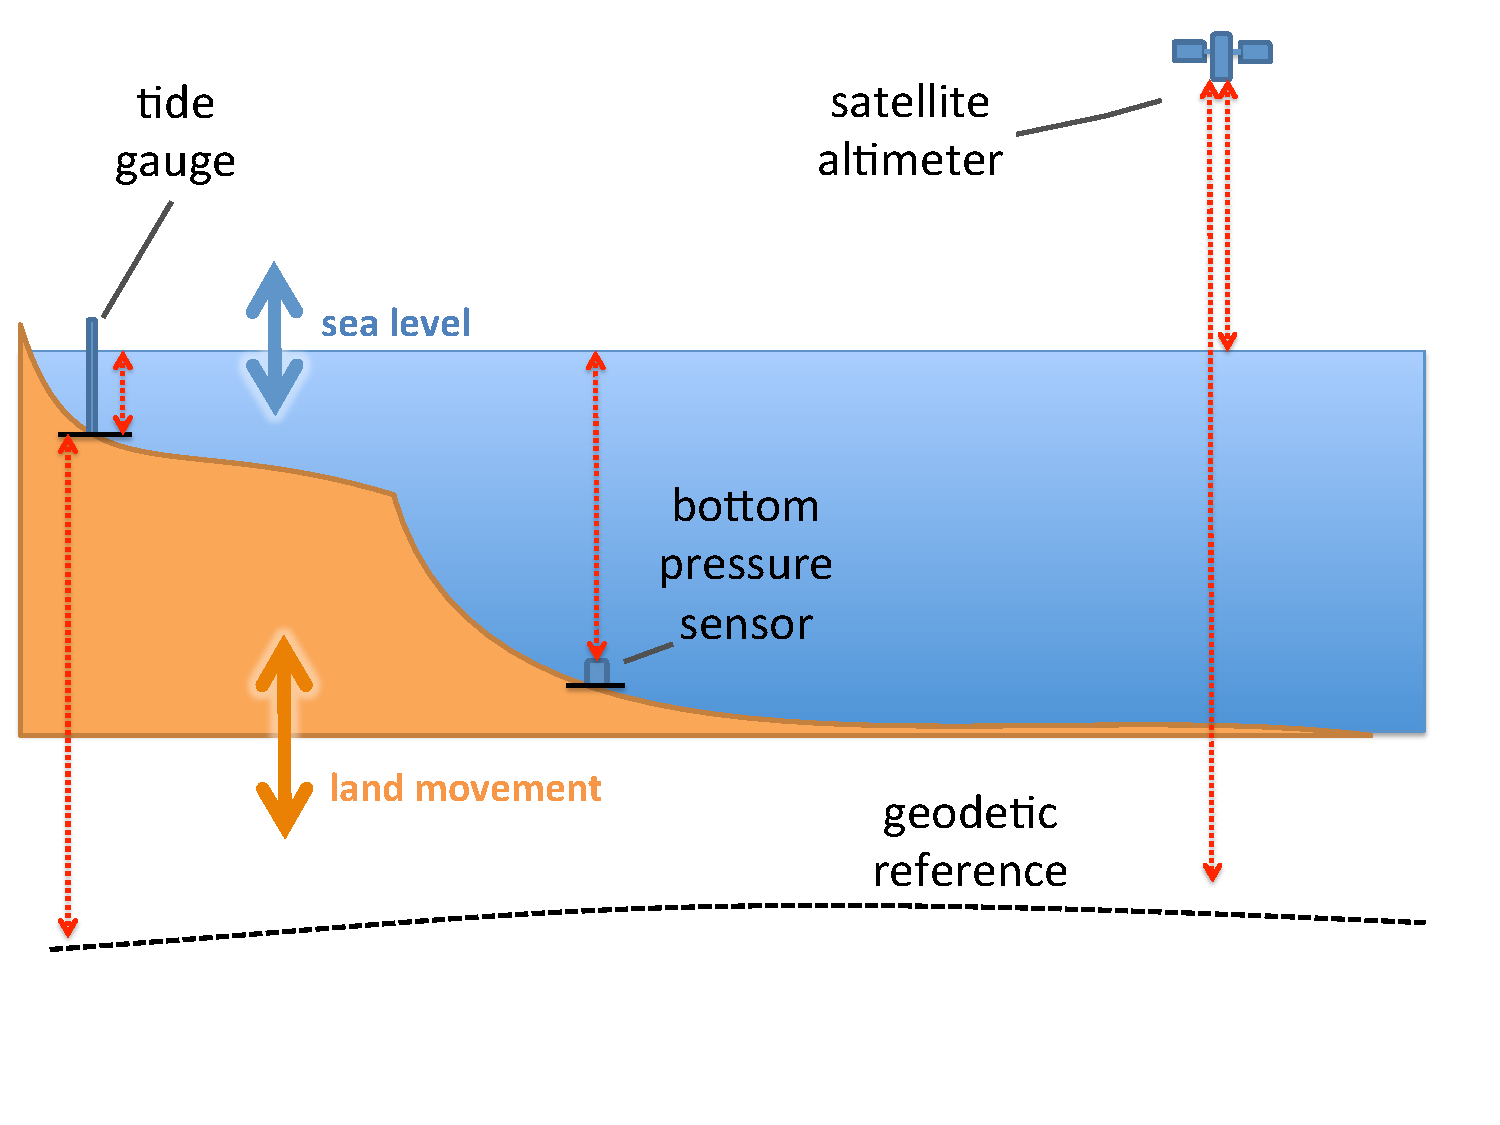
\includegraphics[width=\figwidthBig]{figures/diagrams/sealevel_cartoon.pdf}
  \caption{Schematic illustration of insitu versus remote sea level observations}
  \label{fig:sealevelObsCartoon}
\end{figure}
%-----------------------------
Coastal locations are subject to both global and spatially localised hydrodynamic effects; in addition to influences like sediment movement, riverine phenomena and even coastal engineering works.  The limited extent to which the range of scales present in the tide gauge observations can be adequately represented by any forecast system is a fundamental characterisation discussed across chapters \ref{chp:aggregate},\ref{chp:waveguide} and \ref{chp:tideFlavours}.    
Tide gauge observations can be mapped to certain sea level impacts and decisions, though not always directly; as for instance in \citep{Hague:2019ha}.    The fact that wave run-up and swash are generally invisible to tide gauges is a notable limitation when considering impacts at the land-sea interface \citep{Serafin:2017fl,10.1007/s11069-020-04178-3}.
Commonly tide gauge observations are also the basis of vertical reference information and geodetic derivations that are ultimately connected to the interpretation of any quantitative sea level forecast \citep{Woppelmann:2006un}\citep{AVWS2021}.
More comprehensive observations of sea level than are possible from tide gauges is listed as a key requirement for future development by \citeauthor{10.3389/fmars.2019.00437}.    Video-based systems in particular show promise \citep{10.1175/jtech-d-18-0203.1}\citep{2018agufmep52d..26h} but as yet are far from general oeprational availability. 
%-----------------------------
\begin{figure}[H]\centering
  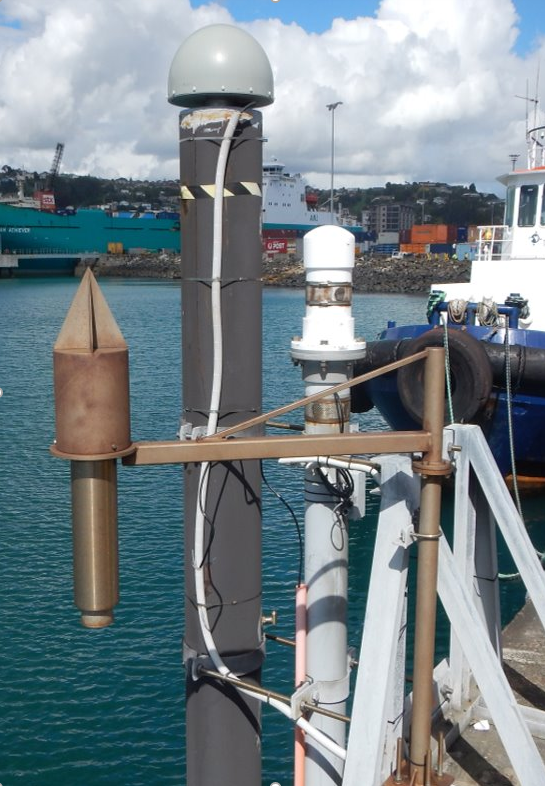
\includegraphics[width=\figwidthThird]{figures/images/tidegaugeEg.png}
  \caption{Typical tide gauge (in fact two) located in a sheltered position; in this case unusually well co-located with a satellite positioning device.}
  \label{fig:tidegauge}
\end{figure}
%-----------------------------

Remote observations of sea level are also derived from what is effectively a very large air-gap .   The derivation from active radar return signals to a meaningful sea level value is non-trivial but very mature away from the coast \citep{Fu:2001ub}.  Operational mesoscale oceanography is heavily dependant on altimeter observations across the global ocean and is discussed further in section \ref{sec:mesoscaleOperational}.  
Operational application of remote sea level observations near the coast is complicated by both the very presence of land within the sensing `footprint' as well as more powerful but shorter time and length scales of sea level variability \citep{Vignudelli:2011wl}.   Whilst this is a  rapidly advancing field, coastal altimetry effectively remains pre-operational and needs to solve the handling of fundamental details such as vertical reference datums \citep{10.3389/fmars.2020.549467}.
The active nadir radar architecture of satellite sea level observations of the last two decades is expected to undergo a qualitative change with the planned wide-swath altimeter missions starting with SWOT \footnote{\url{https://earth.esa.int/web/eoportal/satellite-missions/s/swot}, \url{https://auswot.org/}}.   Wide swath observations of sea level remote observations promise to radically impact water level forecasting in the longer term but can not hope to become operationally relevant for some years to come. 

Operationally-relevant observations of sea level suffer from additional limitations that can be handled differently in more academic settings.   The most basic limitations are whether observations are accessible in near-real-time and the extent to which appropriate metadata is available and up to date.  
Quality control of observations is challenging task that is applied differently between an operational setting as for important long term historical archive projects \footnote{such as \url{www.gloss-sealevel.org}, \url{uhslc.soest.hawaii.edu} and \url{www.gesla.org}}.

The non-uniform network of tide gauges from which sea level observations are provided to the Bureau of Meteorology are operated by a range of port authorities, state agencies and the Bureau itself. Inhomogeneity of tide gauge data quality is expected to persist as a permanent feature for operations; a status that is argued to be a core value of traditional tide prediction services in chapter \ref{chp:tideFlavours}. All evaluations made against tide gauges in this thesis are intentionally based on the Bureau's own operational archive.

%--------------------------------------------------
\section{Unique perspective of the operational setting}
\label{S:operational_setting}

The Australian Bureau of Meteorology is an operational forecasting agency with characteristics that fundamentally frame the present study. The operational setting involves:
\begin{itemize}
    \item a diverse and potentially unknown range of downstream applications;
    \item a suite of geophysical forecasting systems targeting different scales;
    \item regular and continuous schedule of forecast production;
    \item a preference for reliability over fidelity;
    \item reliance on real-time and imperfect observations;
    \item a relatively slow system innovation cycle.
\end{itemize}
This setting provides a perspective on geophysical fluid simulations that thus differs from broader academia as well as commercial forecasts with a clear singular application.   As a result it could be said that this thesis does not launch neatly from a single academic `conversation' in the sense of \citeauthor{Booth:2009vy}, but rather draws on both peer-reviewed literature as well as internal Bureau of Meteorology information where relevant.

The operational setting of the Australian Bureau is considered to share broad characteristics with other national agencies, but detailing the extent to which the findings of this study are generally applicable is non-trivial.    
Unfortunately the documentation of operational systems is partial and inconsistent and can often fall far behind aspirations.  

When considering the suite of forecasting systems that ostensibly forecast sea level variations, there is a basic trade-off between temporal fidelity and prognostic range.    Figure \ref{fig:forecastScalesAll} illustrates this schematically.    The schematic reflects the fact that the physical representation of sea level in a long range climate model intentionally parameterises or excludes phenomena associated with sharp gradients in both space and time in order to provide a very long forecast.  Similarly, simulations that aim to resolve highly local and fast coastal sea level phenomena provide relatively short forecasts.    
(\ref{sec:tidesOverview}.    
\begin{figure}[H]\centering
  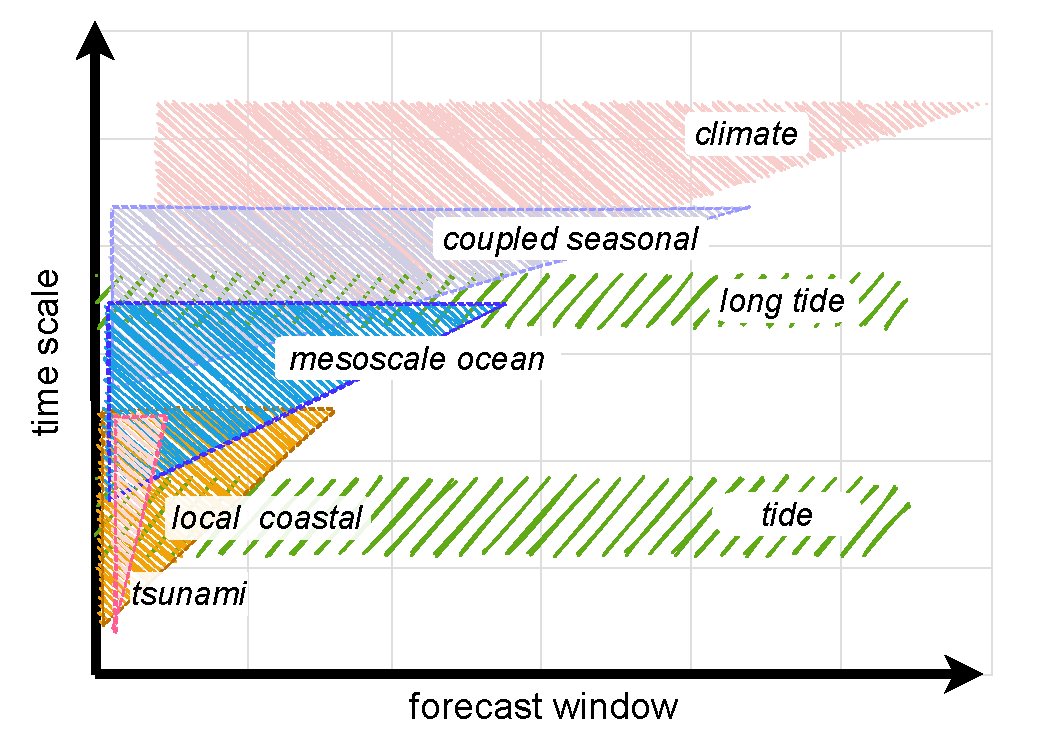
\includegraphics[width=\figwidthBig]{figures/diagrams/scales.pdf}
  \caption{Forecasting suite schematic showing overlapping scales.}
  \label{fig:forecastScalesAll}
\end{figure}
This setting presents a cascade of scales that is arguably the basis for a canonical approach to dynamically forecasting coastal sea level; the lower resolution but longer range systems feed information down to the higher fidelity local forecast.    In fact the realisation of this idealised cascade is limited in the operational setting in part by the incremental historical evolution of the various systems and exasperated by other practical aspects.
For instance, short range forecasts of the potentially extreme storm surges associated with tropical cyclones relies on a simulation framework that takes no account of longer range sea level processes \citep{BRR-031}.   This configuration reasonably focuses on peak sea level signals with magnitudes of several meters and highly localised impacts, but in doing so excludes any role for broader and slower changes that could in principle flow down from the larger-scale forecast systems.

However it is the exceptional status of tide prediction in this framework that is most relevant to the present discussion.  Tidal methods in effect provide a means by which to resolve fast sea level variations with reliable skill independently over unusually long forecast ranges; illustrated by the distinct green shapes in the figure.    This capability reflects the general stationarity of frequency-space patterns associated with the \ATGP{}; as discussed in chapter \ref{sec:tide_intro}.

This unique status of tidal methods with regard to forecast skill and range prompts the problems of conceptual clarity addressed in the body of this thesis.  In short, can we expect the overlap of tidal forecast systems with dynamic physical simulations to be complimentary in a way analogous to the idealised cascade of scales?
%--------------------------------------------------
\subsection{Relevance of restricted scope}
This study is intentionally restricted to \underline{Australia} and the Australian operational setting.  Whilst some characteristics are peculiar and unique to Australia, others are internationally relevant will be discussed as such.


The conceptual scope of the study is intentionally focused on the overlap of tidal methods with the ocean mesoscale and is illustrated schematically in Figure \ref{fig:forecastScalesFocus}.


It is worth emphasising that this focus is well away from the representation of extreme events like tsunami and tropical cyclone surge events.   Plainly, the ability to skillfully forecast such extreme sea level phenomena is of great significance and is relevant to operational forecasting. \citet{McInnes:2016km} provides an overview of sea level extremes as a natural hazard in Australia.    
In fact, the substantial and productive research effort directed to sea level extremes as a hazard has understandably de-prioritised the details of compatibility for forecasts between more mundane sea level fluctuations; and this gap is the focus of the present document. 

This scope also intentionally excludes outputs from nested downscaling of mesoscale forecasts, although these too have some operational applicability.   In fact, a key use of the  \BL{} system is in the provision of open boundary conditions for relocatable regional simulations as described by \citep{10.1080/1755876x.2019.1685834} and \citep{10.1007/978-3-319-15994-2_23}.  As it stands, there is no routine downscaling of mesoscale ocean forecasts carried out operationally by the Australian Bureau of Meteorology; some discussion of prospects is taken up in sections \ref{sec:exploitingPredictability} and  \ref{chp:conclusions}. 

\begin{figure}[H]\centering
  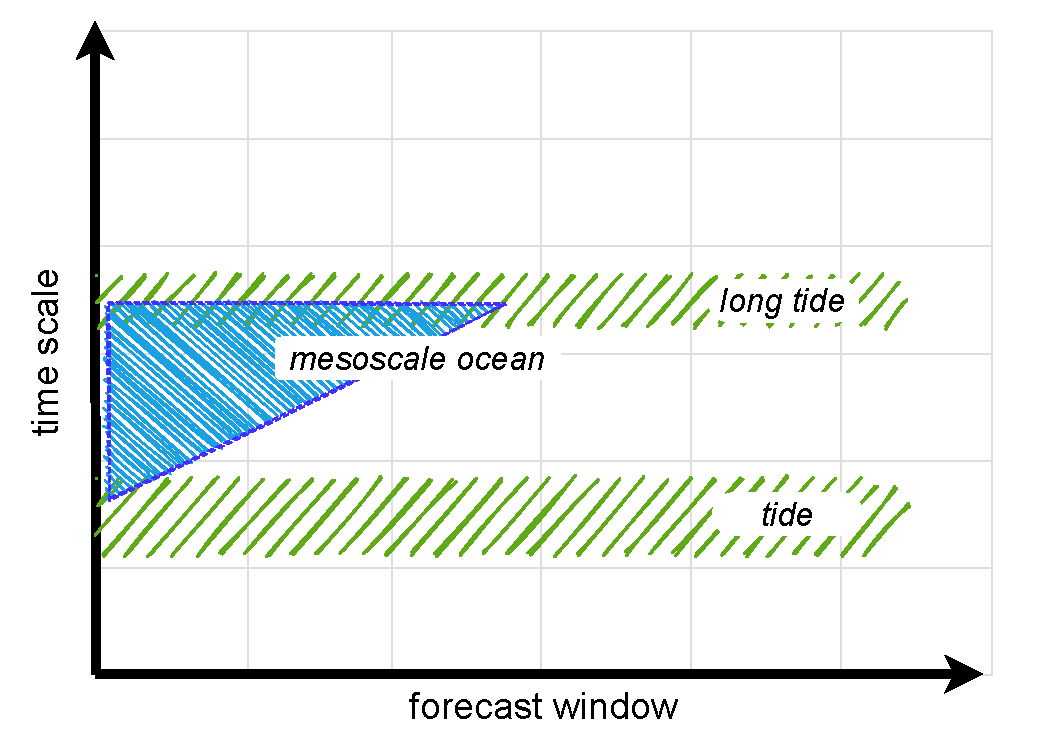
\includegraphics[width=\figwidthBig]{figures/diagrams/scales_focus.pdf}
  \caption{Focus on mesoscale and tidal scales overlap}
  \label{fig:forecastScalesFocus}
\end{figure}

Despite looking away from localised and radical extremes of sea level, the present novel and restricted scope is relevant and important for essentially two  reasons: (1) the are a range of applications in which a longer horizon forecast of essentially ``tidal'' sea level is valued over short range forecast of extremes; and (2) the goal of seamless forecasting will inevitably require conceptual clarity regarding tides to interpret and merge information from numerical systems that are not cleanly complimentary. 

\begin{figure}[H]\centering
  \begin{subfigure}[t]{\figwidthHalf}
      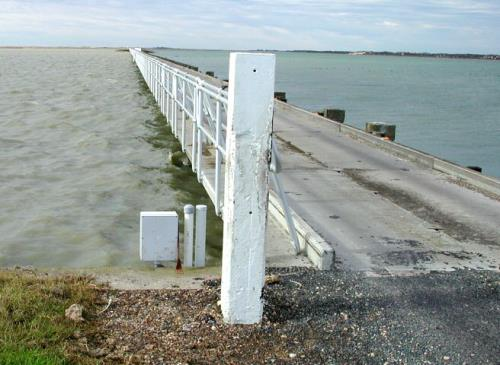
\includegraphics[width=\textwidth]{figures/images/goolwa_ewe_island-environment_sa_gov_au.jpg}
      %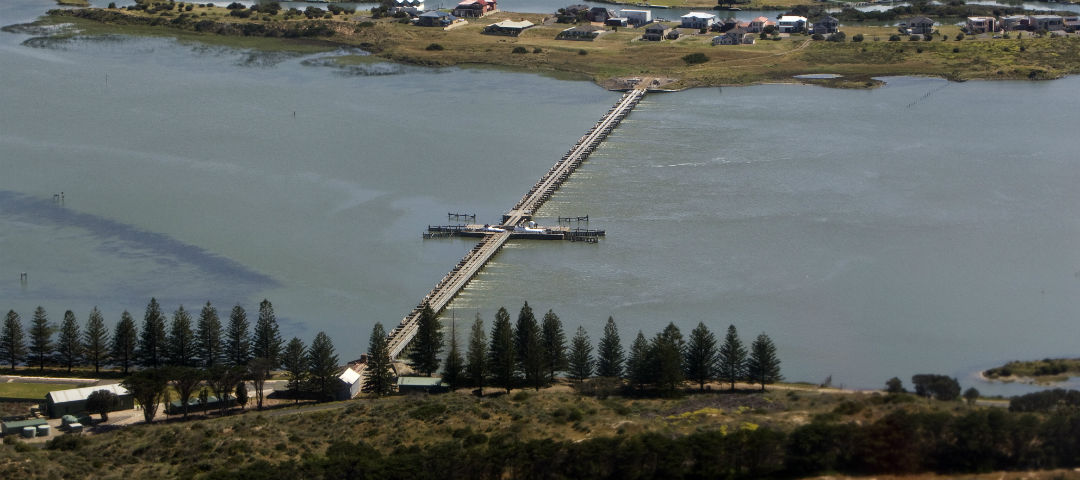
\includegraphics[height=5cm]{figures/images/goolwa-barrage-environment_sa_gov_au.jpg}
      \caption{Coastal infrastructure management. Goolwa barrages in SA are indirectly exposed to ocean sea level. Photo credit Environment SA }
  \end{subfigure}
  \hfill
  \begin{subfigure}[t]{\figwidthHalf}
      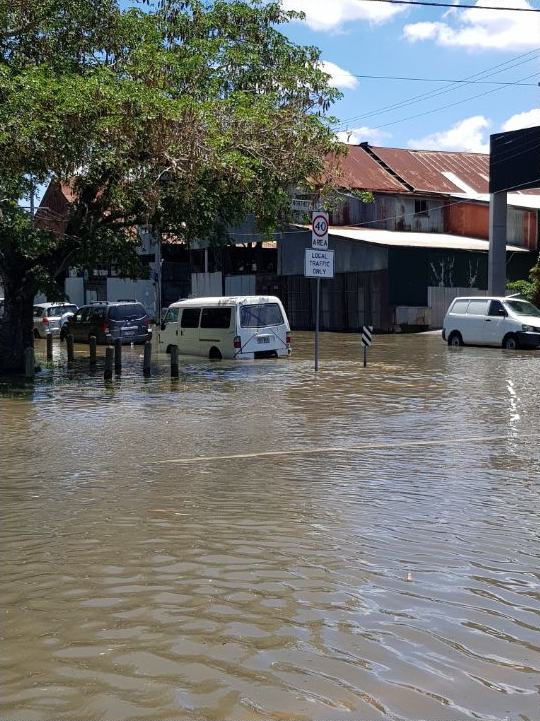
\includegraphics[trim={0 9cm 0 2cm},clip,width=\textwidth]{figures/images/sunnyFlood_ClarkJan2018Brisbane.png}
      %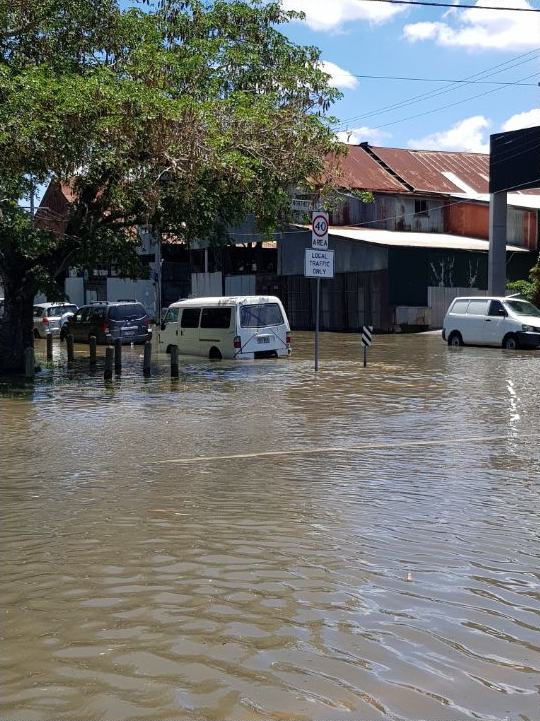
\includegraphics[height=5cm]{figures/images/sunnyFlood_ClarkJan2018Brisbane.png}
      \caption{Nuisance urban flooding associated with predictable compounding of non-extreme sea level events Brisbane 2018. Photo credit Harry Clarke.}
  \end{subfigure}
  \caption{Examples of applications for longer-range routine total sea level forecasts.} 
  \label{fig:applicationPhotos}
\end{figure}


Considering the first reason, applications for non-extreme sea level forecast guidance have a low public profile and generally involve the routine operation of coastal infrastructure or inputs to downstream decision systems.
For instance, consider the management of the estuarine barrages near the mouth of the river Murray in South Australia; one of several structures is shown in Figure \ref{fig:applicationPhotos}.  Here routine multi-day sea level forecasts are one input to decisions regarding the combination of gate closures used to manage flows and salinity in the lower lakes.  
Another context in which longer lead time forecasts are relevant is associated increasing relevance of ``sunny-day'' coastal nuisance flooding \citep{10.1007/s11069-021-04600-4} and compound events more generally \citep{McInnes:2016km}.   Whilst the impacts of such events can be relatively small compared to rare extremes like tsunami, the potential predictability can move  management responses from being reactive into a more planned framework.   
This framework is also applicable to the use of sea level as a input into river level forecasting systems employed bu the Bureau.  For instance where the flow in the lower reaches of a river are parameterised by a tidal-dependant rating table approach a described by \citet{Leahy:2007tx}.


Aside from direct applications, the second reason for given for the relevance of the present scope is as a contribution to the wider goal of developing seamless forecast services; and this is discussed further in the next seciton. 

%--------------------------------------------------
\subsection{Harmonics and seamless forecasts}
\label{sec:concrete}
Over the past decade, the evolution of operational oceanography has increasingly brought dynamic geophysical fluid modelling into the same organisational setting as tide prediction\citep{10.1080/1755876x.2019.1685834};  bringing two perspectives on how to conceptualise and forecast sea level into something akin to the inter-specialist trading zones of  \citet{Galison:1996uc}.  \citet{Jayne:2001tr} for instance highlight the ``vexing problems'' arising from applying frequency-domain tide theory into time-domain ocean simulations.


More broadly, operational forecasting is carried out against a background of ever improving access to real-time earth observations and growing sophistication of numerical simulation across the board.
\citet{Petersen:2012tr} describes the ``general tendency to strive for ever-more-complex models'' that is enabled by increasing computational power , in terms of simulation \emph{concreteness}. Where concreteness of a model is ``defined as the level of aggregation, in terms of both the number of degrees of freedom in the model and the number of processes modelled''.

The Bureau's \textit{Research and Development Plan 2020-2030} places this tendency towards increasingly concrete simulation models within the limitations of operational capacity by describing a trade-off between the four dimensions of resolution, complexity, duration/ensemble size and observations. 
Of special relevance to the present study is the objective of developing seamless services.  ``\textit{Seamless services mean consistent forecasts to users even where the source of the forecast model has changed – for instance, at the transition from ten-day numerical weather prediction to multi-week forecasts}'' \citep{BOM2020}.
Although intuitive enough, designating such a multi-scale service to be ``seamless'' extends the original application of the term from simply an architecture in which to make climate projections \citep{10.1175/bams-87-9-1195}.   


The derivation of seamless services from sea level forecasts raises some unique challenges associated with the qualitatively distinct properties of conventional tide prediction and dynamic fluid simulations.   
Instead of a just managing the transition from higher to lower fidelity with forecast range, a useful seamless sea level forecast will likely need to manage transitions between tide-resolving and tide-excluding simulations against a time-scale-spanning reference tide prediction.  And this transition doesn't fit neatly into what is asserted to be the canonical approach to seamless forecasts whereby increasing forecast horizons are associated with decreasing temporal resolution.   This concept is visualised for discussion in the present thesis by borrowing the chain imagery originally associated with seamless forecasting \citep{10.1175/bams-87-9-1195}.


% mention ROAM and surge ...emphasis why small downscale is great but not the whole answer

Working towards seamless sea level forecasts will thus require conceptual clarity about what constitutes ``tidal'' sea level in each context and means by which to identify, characterise and combine the scales of predictability offered by an evolving but an imperfect suite of operational systems.  
It is the conceptual basis for this goal of seamless sea level forecasting that underpins the sections that follow.
